On se place dans un repère orthonormé \Oij pour l'ensemble de l'exercice.

	\subsection*{Partie A -- Étude d'un cercle}
	\emph{Cette partie est indépendante des parties B et C qui suivent.}

	On considère le cercle $\mathcal{C}$ de centre A$(3 ; 1)$ et de rayon $r = \dfrac{\sqrt{37}}{2}$.

	\begin{center}
		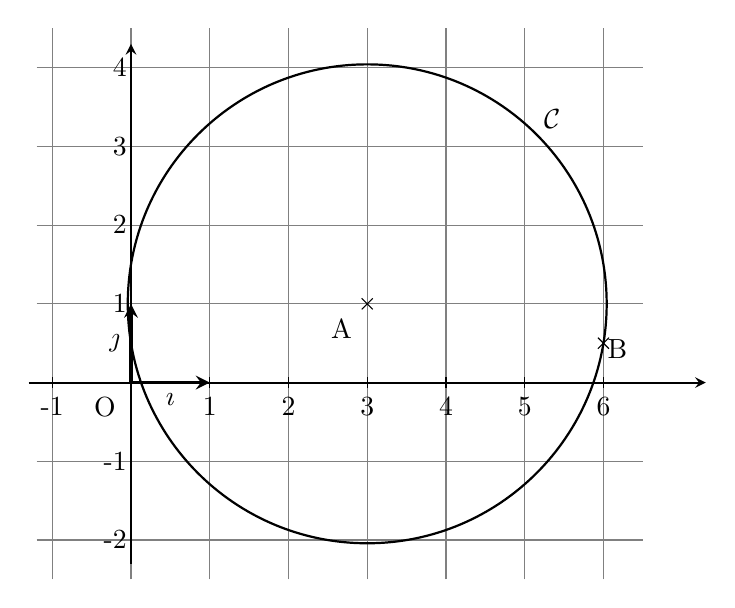
\begin{tikzpicture}[>=stealth]
			\draw[step=1,gray,thin] (-1.2,-2.5) grid (6.5,4.5);
			\draw[->,line width=0.7pt] (-1.3,0) -- (7.3,0);
			\draw[->,line width=0.7pt] (0,-2.3) -- (0,4.3);
			\draw[<->,line width=1.2pt] (1,0) -- (0,0) node[pos=0.5,below]{$\vect{\imath}$}
			--(0,1)node[pos=0.5,left]{$\vect{\jmath}$};
			\node[below left] at (-2pt,-2pt) {O};
			\foreach \x in {-1,1,2,3,4,5,6} \draw (\x,2pt) -- (\x,-2pt) node[below] {\np{\x}};
			\foreach \y in {-2,-1,1,2,3,4} \draw (2pt,\y) -- (2pt,\y) node[left] {\np{\y}};
			\draw[thick] (3,1) circle (3.041);
			\draw[shift={(3,1)}] (-2pt,2pt)--(2pt,-2pt)
			(2pt,2pt)--(-2pt,-2pt)node[below left] {A};
			\draw[shift={(6,0.5)}] (-2pt,2pt)--(2pt,-2pt)
			(2pt,2pt)--(-2pt,-2pt)node[right] {B};
			\node at (5.35,3.35) {$\mathcal{C}$};
		\end{tikzpicture}
	\end{center}

	\begin{minipage}{0.7\linewidth}
		\begin{enumerate}
		\item Justifier que le cercle $\mathcal{C}$ admet pour équation :
		\[ (x-3)^2 + (y-1)^2 = \frac{37}{4}. \]

		\item Démontrer que le point B$(6 ; 0,5)$ appartient au cercle $\mathcal{C}$.
	\end{enumerate}
	\end{minipage}
	\hfill
		\fbox{
			\begin{minipage}{0.25\textwidth}
				\textbf{Aide aux calculs :}\\[0.5em]
				$9{,}25 = \dfrac{37}{4}$\\[0.5em]
				$8{,}75 = \dfrac{35}{4}$\\[0.5em]
				$0{,}5^2 = 0{,}25$
			\end{minipage}
		}

	\vfill
	\begin{center}
		\textbf{TOURNER LA PAGE}
	\end{center}

	\vfill
	~


	Pour la suite de l'exercice, on considère la figure ci-dessous et les données suivantes

	\begin{center}
		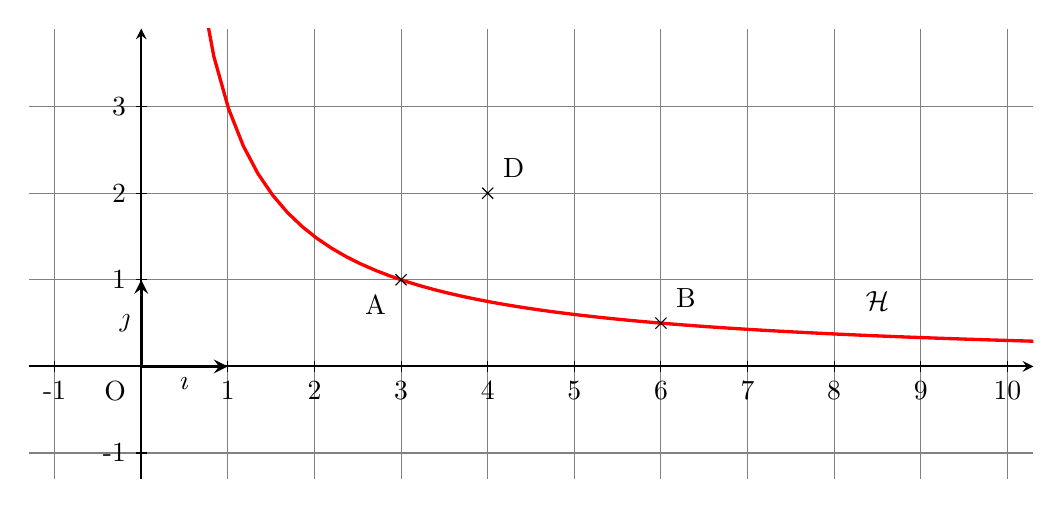
\begin{tikzpicture}[x =11mm, y = 11mm,>=stealth]
			\draw[step=1,gray,thin] (-1.3,-1.3) grid (10.3,3.9);
			\draw[->,line width=0.7pt] (-1.3,0) -- (10.3,0);
			\draw[->,line width=0.7pt] (0,-1.3) -- (0,3.9);
			\draw[<->,line width=1.2pt] (1,0) -- (0,0) node[pos=0.5,below]{$\vect{\imath}$}
			--(0,1)node[pos=0.5,left]{$\vect{\jmath}$};
			\node[below left] at (-2pt,-2pt) {O};
			\foreach \x in {-1,1,2,3,4,5,6,7,8,9,10} \draw (\x,2pt) -- (\x,-2pt) node[below] {\np{\x}};
			\foreach \y in {-1,1,2,3} \draw (2pt,\y) -- (-2pt,\y) node[left] {\np{\y}};
			\clip (-1.3,-1.3) rectangle (10.3,3.9);
			\draw[line width=1.2pt,red] plot[domain=0.5:10.5,samples=60] (\x,{3/\x});
			\draw[shift={(3,1)}] (-2pt,2pt)--(2pt,-2pt)
			(2pt,2pt)--(-2pt,-2pt)node[below left] {A};
			\draw[shift={(6,0.5)}] (-2pt,2pt)--(2pt,-2pt)
			(-2pt,-2pt)--(2pt,2pt)node[above right] {B};
			\draw[shift={(4,2)}] (-2pt,2pt)--(2pt,-2pt)
			(-2pt,-2pt)--(2pt,2pt)node[above right] {D};
			\node at (8.5,0.75) {$\mathcal{H}$};
		\end{tikzpicture}
	\end{center}

	\begin{itemize}[label = \textbullet~]
		\item l'équation de la courbe $\mathcal{H}$ est : \quad $y = \dfrac{3}{x}$ \quad pour $x$ strictement positif ;

		\item les coordonnées des points sont : A$(3 ; 1)$, B$(6 ; 0,5)$ et D$(4 ; 2)$.
	\end{itemize}

	On considère un point M mobile sur la courbe $\mathcal{H}$, d'abscisse $x>0$.

	L'objectif des deux parties suivantes est de démontrer qu'il n'existe qu'un seul point $M$ tel que l'angle $\widehat{\mathrm{DAM}}$ soit droit.

	\subsection*{Partie B -- Étude d'un cas particulier}

	\begin{enumerate}
		\item Justifier que le point B appartient à la courbe $\mathcal{H}$.
		\item \begin{enumerate}
			\item Déterminer les coordonnées des vecteurs $\vectt{AD}$ et $\vectt{AB}$.

			\item En déduire le produit scalaire $\vectt{AD}\cdot\vectt{AB}$.

			\item L'angle $\widehat{\mathrm{DAB}}$ est-il droit ?

			Justifier.
		\end{enumerate}
	\end{enumerate}

	\subsection*{Partie C -- Étude du cas général}

	\begin{enumerate}
		\item Résoudre dans $\R$ l'équation \quad $x^2 - 4x + 3 = 0$.
		\item On rappelle que M est un point sur la courbe $\mathcal{H}$ d'abscisse $x>0$.

		Démontrer qu'il n'existe qu'un seul point M tel que l'angle $\widehat{\mathrm{DAM}}$ est droit.
	\end{enumerate}

	\vspace{1em}
	\emph{Toute trace de recherche pourra être valorisée.}
